\documentclass[tikz,border=12pt]{standalone}
\usetikzlibrary{patterns}
\begin{document}
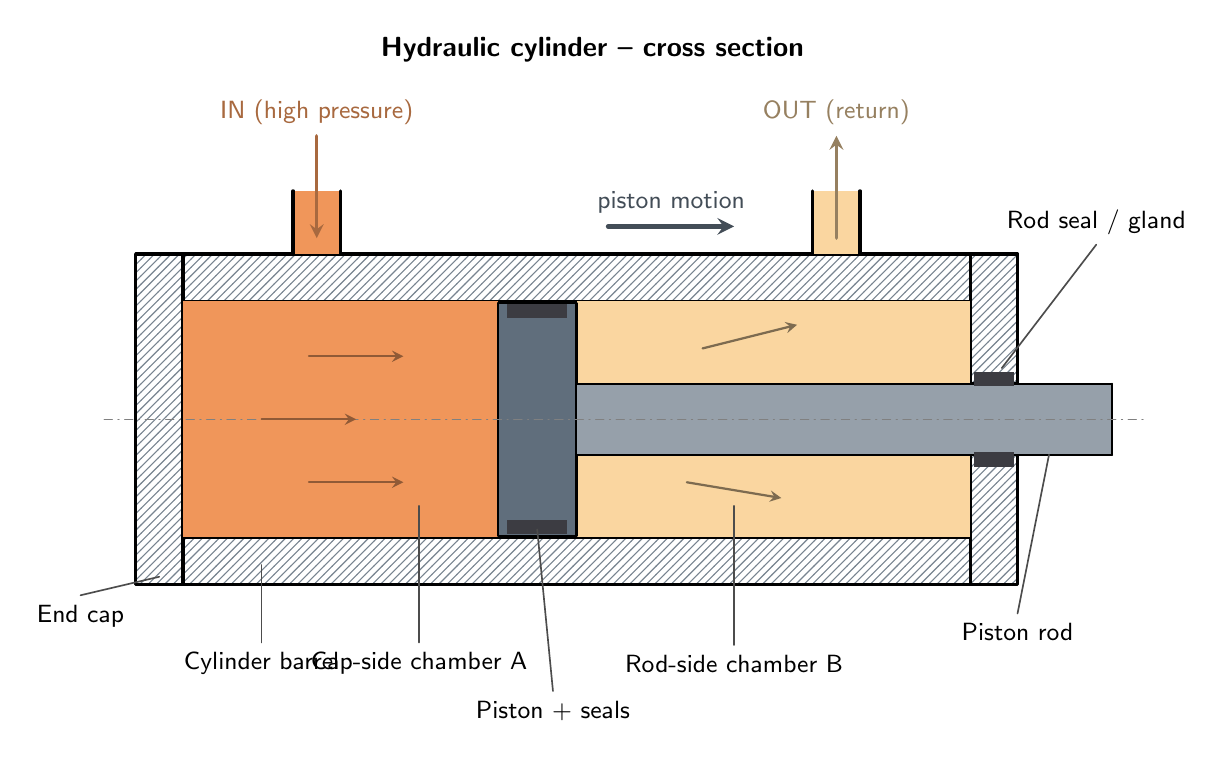
\begin{tikzpicture}[line cap=round,line join=round,>=stealth,
  lbl/.style={font=\small\sffamily},
  leader/.style={gray!60!black,semithick}]
  \definecolor{steel}{RGB}{176,186,196}
  \definecolor{steeldark}{RGB}{120,132,144}
  \definecolor{oilhi}{RGB}{240,150,90}
  \definecolor{oillo}{RGB}{250,214,160}
  \definecolor{piston}{RGB}{96,110,124}
  \definecolor{rodcol}{RGB}{150,160,170}
  \definecolor{seal}{RGB}{60,60,66}

  % ---- cylinder cross-section ----
  % outer walls (hatched section)
  \fill[pattern=north east lines,pattern color=steeldark]
    (0,3.0) rectangle (10.0,3.6);
  \fill[pattern=north east lines,pattern color=steeldark]
    (0,-0.6) rectangle (10.0,0.0);
  \draw[very thick] (0,3.0) -- (10.0,3.0);
  \draw[very thick] (0,0.0) -- (10.0,0.0);
  \draw[very thick] (0,3.6) -- (10.0,3.6);
  \draw[very thick] (0,-0.6) -- (10.0,-0.6);
  % left end cap
  \fill[pattern=north east lines,pattern color=steeldark] (-0.6,-0.6) rectangle (0,3.6);
  \draw[very thick] (-0.6,-0.6) rectangle (0,3.6);
  % right end cap with rod hole
  \fill[pattern=north east lines,pattern color=steeldark] (10.0,1.95) rectangle (10.6,3.6);
  \fill[pattern=north east lines,pattern color=steeldark] (10.0,-0.6) rectangle (10.6,1.05);
  \draw[very thick] (10.0,1.95) rectangle (10.6,3.6);
  \draw[very thick] (10.0,-0.6) rectangle (10.6,1.05);

  % chambers
  \fill[oilhi] (0,0) rectangle (4.0,3.0);   % cap side (high pressure)
  \fill[oillo] (5.0,0) rectangle (10.0,3.0); % rod side (low pressure)

  % piston
  \fill[piston] (4.0,0.02) rectangle (5.0,2.98);
  \fill[seal] (4.12,2.78) rectangle (4.88,2.96);
  \fill[seal] (4.12,0.04) rectangle (4.88,0.22);
  \draw[thick] (4.0,0.02) rectangle (5.0,2.98);

  % rod
  \fill[rodcol] (5.0,1.05) rectangle (11.8,1.95);
  \draw[thick] (5.0,1.05) -- (11.8,1.05) (5.0,1.95) -- (11.8,1.95);
  \draw[thick] (11.8,1.05) -- (11.8,1.95);
  % rod seal at end cap
  \fill[seal] (10.05,1.92) rectangle (10.55,2.1);
  \fill[seal] (10.05,0.9) rectangle (10.55,1.08);

  % center line
  \draw[gray,dash dot] (-1.0,1.5) -- (12.2,1.5);

  % ---- ports and flow arrows ----
  % port A (cap side, inflow)
  \fill[oilhi] (1.4,3.6) rectangle (2.0,4.4);
  \draw[very thick] (1.4,3.6) -- (1.4,4.4) (2.0,3.6) -- (2.0,4.4);
  \draw[->,very thick,oilhi!70!black] (1.7,5.1) -- (1.7,3.8);
  \node[lbl,oilhi!70!black] at (1.7,5.4) {IN (high pressure)};
  % port B (rod side, outflow)
  \fill[oillo] (8.0,3.6) rectangle (8.6,4.4);
  \draw[very thick] (8.0,3.6) -- (8.0,4.4) (8.6,3.6) -- (8.6,4.4);
  \draw[->,very thick,oillo!60!black] (8.3,3.8) -- (8.3,5.1);
  \node[lbl,oillo!60!black] at (8.3,5.4) {OUT (return)};

  % flow arrows inside chambers
  \draw[->,thick,oilhi!60!black] (1.0,1.5) -- (2.2,1.5);
  \draw[->,thick,oilhi!60!black] (1.6,2.3) -- (2.8,2.3);
  \draw[->,thick,oilhi!60!black] (1.6,0.7) -- (2.8,0.7);
  \draw[->,thick,oillo!50!black] (6.6,2.4) -- (7.8,2.7) ;
  \draw[->,thick,oillo!50!black] (6.4,0.7) -- (7.6,0.5);

  % piston motion arrow
  \draw[->,ultra thick,piston!70!black] (5.4,3.95) -- (7.0,3.95);
  \node[lbl,piston!70!black] at (6.2,4.25) {piston motion};

  % ---- labels with leader lines ----
  \node[lbl] (cyl) at (1.0,-1.6) {Cylinder barrel};
  \draw[leader] (cyl.north) -- (1.0,-0.35);
  \node[lbl] (cap) at (-1.3,-1.0) {End cap};
  \draw[leader] (cap.north) -- (-0.3,-0.5);
  \node[lbl] (cha) at (3.0,-1.6) {Cap-side chamber A};
  \draw[leader] (cha.north) -- (3.0,0.4);
  \node[lbl] (pis) at (4.7,-2.2) {Piston + seals};
  \draw[leader] (pis.north) -- (4.5,0.1);
  \node[lbl] (chb) at (7.0,-1.6) {Rod-side chamber B};
  \draw[leader] (chb.north) -- (7.0,0.4);
  \node[lbl] (rod) at (10.6,-1.2) {Piston rod};
  \draw[leader] (rod.north) -- (11.0,1.05);
  \node[lbl] (gl) at (11.6,4.0) {Rod seal / gland};
  \draw[leader] (gl.south) -- (10.4,2.15);

  % title
  \node[font=\sffamily\bfseries] at (5.2,6.2) {Hydraulic cylinder -- cross section};
\end{tikzpicture}
\end{document}
